\part{Trace-Determinant-Plane}
\lecture{Trace-Determinant Plane}{Trace-Determinant-Plane}
\section{Trace-Determinant Plane}


\title{Ordinary Differential Equations}
\subtitle{Math 232 - The Trace Determinant Plane}
\date{7 November 2012}

\begin{frame}
  \titlepage
\end{frame}

\begin{frame}
  \frametitle{Outline}
  \tableofcontents[pausesection,hideothersubsections]
\end{frame}


\subsection{Behavior of Solutions to DEs}


\begin{frame}
  \frametitle{Behavior of Solutions to DEs}

  The eigenvalues determine the stability characteristics of the
  system of DEs.

  If the eigenvalues are \blueText{real}:
  \begin{itemize}
  \item $\lambda_2 < \lambda_1 < 0$ - Sink
  \item $\lambda_2 < 0 < \lambda_1$ - Saddle
  \item $0 < \lambda_2 < \lambda_1$ - Source
  \end{itemize}

  If the eigenvalues are \blueText{complex}, $\lambda_{1,2}=\redText{a}+ib$:
  \begin{itemize}
  \item $\redText{a}<0$ - Attracting spiral
  \item $\redText{a}>0$ - Repelling spiral
  \item $\redText{a}=0$ - Center
  \end{itemize}

\end{frame}

\iftoggle{clicker}{%
\begin{frame}
  \frametitle{Clicker Quiz}

   \ifnum\value{clickerQuiz}=1{%
   The matrix for a  system of equations,
   \begin{eqnarray*}
     \deriv{~}{t} \vec{x} & = & A \vec{x},
   \end{eqnarray*}
   has eigenvalues $\lambda_1=-2+\sqrt{3}i$ and
   $\lambda_1=-2-\sqrt{3}i$. What is the general behavior of the
   resulting system?

     \begin{tabular}{ll}
       A: &  Source \\
       B: &  Sink \\
       C: &  Spiral Source \\
       D: &  Spiral Sink
     \end{tabular}

     \vfill


 }\fi

 \ifnum\value{clickerQuiz}=2{%

   The matrix for a  system of equations,
   \begin{eqnarray*}
     \deriv{~}{t} \vec{x} & = & A \vec{x},
   \end{eqnarray*}
   has eigenvalues $\lambda_1=2+\sqrt{3}i$ and
   $\lambda_1=2-\sqrt{3}i$. What is the general behavior of the
   resulting system?

     \begin{tabular}{ll}
       A: &  Source \\
       B: &  Sink \\
       C: &  Spiral Source \\
       D: &  Spiral Sink
     \end{tabular}

     \vfill

 }\fi

 \ifnum\value{clickerQuiz}=3{%
  \vfill
 }\fi
\end{frame}
}


\subsection{Special Case of $2\times 2$ Systems}

\begin{frame}
  \frametitle{Special Case of $2\times 2$ Systems}

  \begin{eqnarray*}
    \deriv{~}{t} \vec{x} & = & \arrayTwo{a}{b}{c}{d} \vec{x}, \\
    & = & A \vec{x}.
  \end{eqnarray*}

  \uncover<2->
  {
    Find the eigenvalues:
    \begin{eqnarray*}
      \only<2>
      {
        \det\lp\arrayTwo{a-\lambda}{b}{c}{d-\lambda}\rp & = & 
        \lambda^2 - \redText{(a+d)}
        \lambda + \blueText{(ad-bc)}, \\
      }
      \only<3->
      {
        \det\lp\arrayTwo{a-\lambda}{b}{c}{d-\lambda}\rp & = & 
        \lambda^2 - \underbrace{\redText{(a+d)}}_{\mathrm{call~this~T}}
        \lambda + \underbrace{\blueText{(ad-bc)}}_{\mathrm{call~this~D}}, \\
      }
      \uncover<4->{& = & \lambda^2 - \redText{T}\lambda + \blueText{D}.}
    \end{eqnarray*}
  }

  \uncover<5->
  {
    \begin{eqnarray*}
      \Rightarrow \lambda_{1,2} & = & \frac{T\pm\sqrt{T^2-4D}}{2}.
    \end{eqnarray*}
  }


\end{frame}


\begin{frame}
  \frametitle{Different Cases}

  If $T^2-4D>0$
  \begin{itemize}
  \item $T<0$ and $D>0$ - Sink
  \item $T<0$ and $D<0$ - Saddle
  \item $T>0$ and $D<0$ - Saddle
  \item $T>0$ and $D>0$ - Source
  \end{itemize}

  If $T^2-4D<0$ - Complex case:
  \begin{itemize}
  \item $T<0$ - Attracting Spiral
  \item $T=0$ - Centered
  \item $T>0$ - Repelling Spiral
  \end{itemize}


\end{frame}

\begin{frame}
  \frametitle{Trace-Determinant Plane}

  \only<1>{\centerline{\includegraphics[width=5cm]{img/traceDeterminant}}}

  \only<2->{\centerline{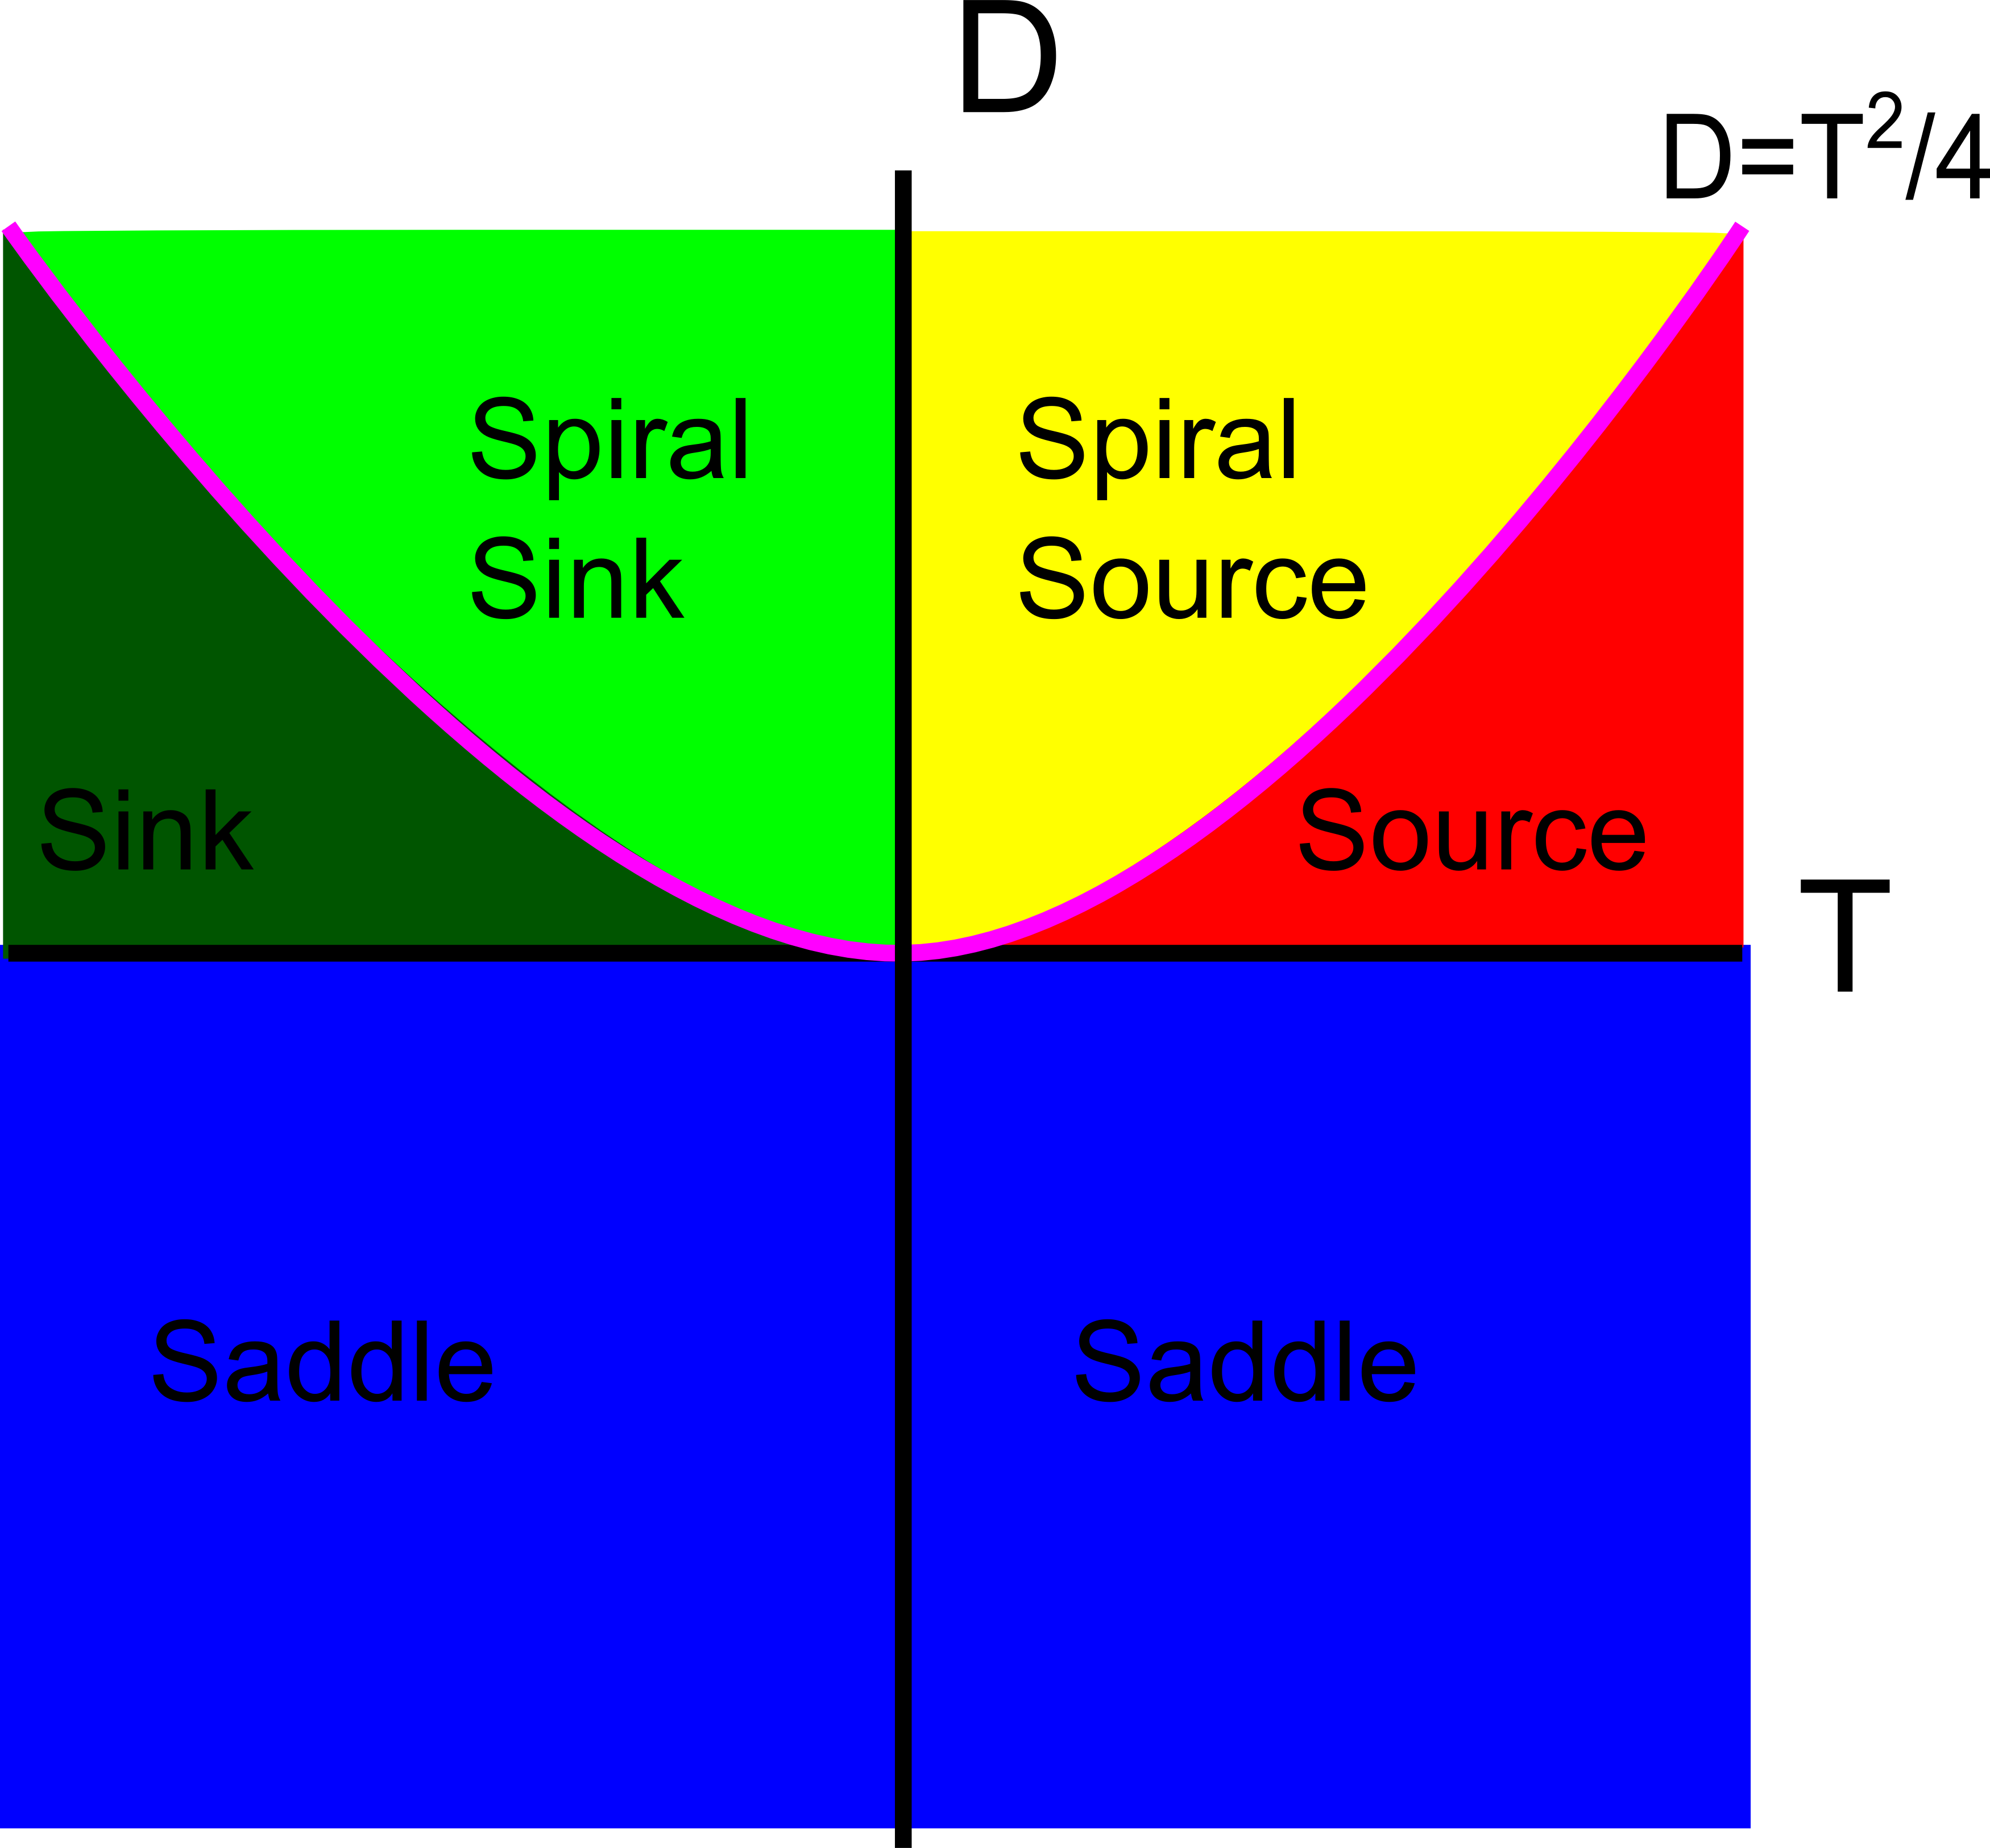
\includegraphics[width=5cm]{img/traceDeterminantAnnotated}}}
  
\end{frame}

\subsection{Examples}

\begin{frame}
  \frametitle{Example}

  \begin{eqnarray*}
    \deriv{~}{t} \vec{x} & = & \arrayTwo{2}{4}{1}{3} \vec{x}.
  \end{eqnarray*}

\end{frame}


\iftoggle{clicker}{%
\begin{frame}
  \frametitle{Clicker Quiz}

   \ifnum\value{clickerQuiz}=1{%
   What are the values of $D$ and $T$ for the system of equations
   given by
   \begin{eqnarray*}
     \deriv{~}{t} \vec{x} & = & \arrayTwo{1}{4}{1}{3} \vec{x}?
   \end{eqnarray*}

     \begin{tabular}{ll}
       A: &   $D=7$, $T=4$ \\
       B: &   $D=-1$, $T=4$ \\
       C: &   $D=-1$, $T=3$ \\
     \end{tabular}

     \vfill


 }\fi

 \ifnum\value{clickerQuiz}=2{%
   What are the values of $D$ and $T$ for the system of equations
   given by
   \begin{eqnarray*}
     \deriv{~}{t} \vec{x} & = & \arrayTwo{1}{4}{1}{3} \vec{x}?
   \end{eqnarray*}

     \begin{tabular}{ll}
       A: &   $D=-1$, $T=3$ \\
       B: &   $D=-1$, $T=4$ \\
       C: &   $D=7$, $T=4$ \\
     \end{tabular}

     \vfill

 }\fi

 \ifnum\value{clickerQuiz}=3{%
  \vfill
 }\fi
\end{frame}
}


\begin{frame}
  \frametitle{Example}

  \begin{eqnarray*}
    \deriv{~}{t} \vec{x} & = & \arrayTwo{1}{4}{1}{3} \vec{x}.
  \end{eqnarray*}

\end{frame}


\begin{frame}
  \frametitle{Example}

  What is the behavior of
  \begin{eqnarray*}
    \deriv{~}{t} \vec{x} & = & \arrayTwo{1}{k}{1}{0} \vec{x}.
  \end{eqnarray*}
  for all values of $k$?
  

\end{frame}


\begin{frame}
  \frametitle{Example}

  What is the behavior of
  \begin{eqnarray*}
    \deriv{~}{t} \vec{x} & = & \arrayTwo{-2}{k}{k}{0} \vec{x}.
  \end{eqnarray*}
  for all values of $k$?


\end{frame}


\begin{frame}
  \frametitle{Example}

  What is the behavior of
  \begin{eqnarray*}
    \deriv{~}{t} \vec{x} & = & \arrayTwo{1}{k}{1}{-2} \vec{x}.
  \end{eqnarray*}
  for all values of $k$?


\end{frame}


\begin{frame}
  \frametitle{Example}

  What is the behavior of
  \begin{eqnarray*}
    \deriv{~}{t} \vec{x} & = & \arrayTwo{k}{2}{-1}{0} \vec{x}.
  \end{eqnarray*}
  for all values of $k$?


\end{frame}




% LocalWords:  Clarkson pausesection hideothersubsections
